% 
% Annual CCN conference
% Sample LaTeX Two-Page Summary -- Proceedings Format
% based on the prior cognitive science style file

% Original : Ashwin Ram (ashwin@cc.gatech.edu)       04/01/1994
% Modified : Johanna Moore (jmoore@cs.pitt.edu)      03/17/1995
% Modified : David Noelle (noelle@ucsd.edu)          03/15/1996
% Modified : Pat Langley (langley@cs.stanford.edu)   01/26/1997
% Latex2e corrections by Ramin Charles Nakisa        01/28/1997 
% Modified : Tina Eliassi-Rad (eliassi@cs.wisc.edu)  01/31/1998
% Modified : Trisha Yannuzzi (trisha@ircs.upenn.edu) 12/28/1999 (in process)
% Modified : Mary Ellen Foster (M.E.Foster@ed.ac.uk) 12/11/2000
% Modified : Ken Forbus                              01/23/2004
% Modified : Eli M. Silk (esilk@pitt.edu)            05/24/2005
% Modified : Niels Taatgen (taatgen@cmu.edu)        10/24/2006
% Modified : David Noelle (dnoelle@ucmerced.edu)     11/19/2014
% Modified : Konrad Kording (koerding@gmail.com)     2/15/2017
% Modified : Thomas Naselaris (tnaselar@gmail.com)   3/18/2022

\documentclass[10pt,letterpaper]{article}

\usepackage{ccn}
\usepackage{pslatex}
\usepackage[natbibapa]{apacite} % apacite with natbib's \citet / \citep; do not also load natbib
\usepackage{graphicx}
\usepackage{float}
\usepackage{array}
\usepackage{pdfpages}
\graphicspath{{./}{../}} 

\usepackage{url}            % simple URL typesetting
\usepackage{booktabs}       % professional-quality tables
\usepackage{amsfonts}       % blackboard math symbols
\usepackage{nicefrac}       % compact symbols for 1/2, etc.
\usepackage{microtype}      % microtypography
\usepackage{xcolor}         % colors
\usepackage{amsmath}
\usepackage{amssymb}
\usepackage{mathtools}
\usepackage{amsthm}
\usepackage{svg}
\usepackage[labelfont=bf, margin=0.8cm, font=sf]{caption}
% \usepackage[margin=0.5in]{geometry}
\usepackage{hyperref}       % hyperlinks; load last
\hypersetup{colorlinks=true, linkcolor=blue!60!black, citecolor=blue!60!black, urlcolor=blue!60!black}

\title{Does Distance Preservation Explain Grid Cells? Reviewing Xu et al. (ICLR 2025)}
 
\author{{\large \bf Karabelo Borotho } \\ University of the Witwatersrand, 1 Jan Smuts Ave,\\ Braamfontein, Johannesburg, 2000, South Africa
  \AND {\large \bf Nabeel Mahomed } \\ University of the Witwatersrand, 1 Jan Smuts Ave,\\ Braamfontein, Johannesburg, 2000, South Africa}


\begin{document}

\maketitle
\phantom{.}
\newpage
\phantom{.}
\newpage
% \section{Abstract}
% {
% \bf
% \looseness=-1
% Roughly 20 lines. It should follow the format of the paper where each section is summarised as a sentence (not a fixed rule but a bit of a heuristic).
% }
% \begin{quote}
% \small
% \textbf{Keywords:} 
% 3 Words or phrases that give the main categories or topics of the work
% \end{quote}

\section{Summary} \label{Summary}
\looseness=-1
%See project brief for description of each section. You may use figures or tables from the paper you are reviewing to make your point. You can put them in the Appendix and reference them here. For example, I could draw your attention to Figure~\ref{fig:wave} or Table~\ref{tab:nonlin}.%
Building on the conformal isometry hypothesis proposed by prior models and isolating grid cells by removing place cells entirely, this paper tests whether that hypothesis, with minimal extra assumptions, is enough to produce hexagonal firing. The model learns the population activity of $d = 24$ grid cells as a vector $v(x)$ at each position, plus a transformation $F$ (the “RNN”) that predicts $v(x + \Delta x)$ from $v(x)$. This neural space, while intrinsically flat, is a curved manifold, and so cannot preserve distance exactly beyond small steps; the paper minimises this error with a two-part loss for the conformal isometry error between spaces and the positional transformation through an RNN, while normalisation and non-negativity are enforced after each training step. Ultimately, the paper shows that hexagonal firing patterns are reproducible from the conformal isometry hypothesis together with a transformation model and normalisation, and argues theoretically that the hexagonal flat torus is the most distance-preserving. The paper reports hexagons for the linear and both nonlinear forms of $F$. Every solution is a torus, and only the hexagonal one has an isometry error that is the same in all directions, which makes it minimal. Finally, the distance relationship in recorded rat grid cells \citep{gardner2021toroidal} is compared with the simulation and found to be approximately consistent. 

\section{Originality} \label{sec:originality}
The normative origin of hexagonal firing fields in medial entorhinal cortex (MEC) grid cells remains a central debate in computational neuroscience. Existing models in the literature generally fall into three paradigms:
\begin{enumerate}
    \item \textbf{Continuous Attractor Neural Networks (CANNs)}, which hand-engineer recurrent synaptic weight matrices on pre-defined neural sheets.
    \item \textbf{Task-Driven RNNs}, which optimize for spatial path integration or place-cell prediction, though later critiques argue that hexagonal grids often fail to emerge without sensitive hyperparameter tuning.
    \item \textbf{Basis Expansion \& Non-Negative PCA} (including the model of Sorscher and colleagues that appears as one of the paper's Table~1 baselines), which derive grid patterns from place-cell inputs under non-negativity constraints, but rely on predefined center-surround (Difference-of-Gaussian) place-cell tuning profiles whose biological plausibility is debated.
\end{enumerate}

The authors build directly upon the conformal isometry framework introduced by \citet{gao2021path} and extended in follow-up work by the same group. While earlier conformal models trained grid cells together with place-cell inputs, the authors achieve scientific reductionism by isolating a single grid cell module without place-cell inputs. 

The closest methodological comparison in recent literature is \citet{dorrell2023actionable}, who similarly derive grid-like representations from minimal normative action constraints without place-cell scaffolding. Comparing levels of generality against Dorrell et al.\ reveals a key tradeoff:

The authors provide a \emph{more general} framework regarding transition dynamics, reporting grid formation across linear and diverse non-linear recurrent networks (ReLU, GELU, Tanh, Leaky ReLU, Swish).

Conversely, the authors present a \emph{less general} model regarding scale and modularity. While Dorrell et al.\ naturally yield multiple grid modules from their optimization formulation, the authors require fixing an explicit target scaling factor $s$ \emph{a priori} for each single module, lacking an intrinsic mechanism to self-generate multi-scale modularity without re-introducing place-cell decoders.

\subsubsection{Strengths}
Isolating the grid cell module shows that hexagonal patterns can arise from distance preservation alone, without place-cell tuning. Furthermore, the paper reports grid formation across five activation functions, although in our reproduction the nonlinear model was hexagonal on only 1 of 2 seeds.
\subsubsection{Weaknesses}
The model relies on a one-step loss function $L_2$ rather than backpropagation through time (BPTT), omitting multi-step recurrent trajectory dynamics. Additionally, enforcing population norm normalization ($\|v(x)\|=1$) after every optimization step artificially constrains the neural manifold to prevent scalar drift.

The authors select a highly abstract, single-module setting. This abstraction level is well-justified for the paper's core research question: by stripping away inter-modular coupling and place-cell inputs, the authors isolate the metric objective, making the 4th-order Taylor expansion proof mathematically tractable. While this choice omits biological complexities such as rate remapping or boundary shearing, it successfully establishes a clean, rigorous theoretical baseline for spatial representation theory.

\section{Clarity} \label{sec:clarity}
The paper is clearly written and well structured. The conformal isometry hypothesis is introduced with a single equation and an intuitive example of the scaling factor as a unit of measurement (\S2.3), so a reader without a background in differential geometry can follow the central idea before any formal machinery appears. The four assumptions are each stated in one line and mapped directly to a loss term or a projection (\S 3.1–3.2), which makes the model easy to reconstruct conceptually. Figures earn their place: the paper's Figure 1 acts as a fitting summary of the main concepts behind conformal isometry and the transformations addressed in the paper, Figure 2 shows the learned response maps across scaling factors alongside the toroidal analysis of the population code, and Figure 4 turns the curvature argument into a single plot of neural against physical distance. The main theoretical results (Propositions 1 and 4, Theorems 5 and 6) are proven in the main text, with supporting lemmas deferred to Appendix C, so the argument stays rigorous without losing its flow. The main weaknesses are in the numerical detail. The value of $\lambda$, the number of heading directions and the initialisation are never given, and $\Delta x$ is described only as “uniform” without saying whether it is uniform over the disc of displacements or in length (\hyperref[sec:repro]{Reproducibility}, Table~\ref{tab:choices}). Gridness and grid scale are cited rather than defined, and the criterion behind “valid rate” is never stated. Figure captions are largely self-contained, stating the model and scaling factor for each panel, although Table 1's caption is not: it attributes each row to its model’s authors but does not say where the baseline values come from, how many runs underlie each value, or which gridness threshold defines a valid grid cell. 

\section{Quality} \label{sec:quality}
%Please remember to comment on the level of abstraction chosen for the model and how this ties to the research question throughout the review.%
The scientific approach is sound overall, with gaps that could be closed by additional experiments rather than a change of method. The choice of abstraction suits the research question. The paper asks whether conformal isometry is sufficient to produce hexagonal grid patterns, and that can only be tested by removing other possible causes, mainly the place-cell input that earlier models rely on. Rather than explaining how the hippocampal circuit actually produces grid cells, the model offers a candidate principle the circuit could implement, which future work can then test against models that reintroduce place cells and against recordings. The ablations are a particular strength: each assumption is removed in turn, which the paper uses to argue that conformal isometry, the transformation model and normalisation are each necessary, while non-negativity is not; our reproduction supports this only in part (\hyperref[sec:released]{Reproducibility}).

Three weaknesses limit how strongly the results support the claims. First, the robustness of the main result is not demonstrated. The paper reports a 100\% valid rate without stating how many training runs it is based on or how much results vary between them. In our reproduction, following the paper’s description, hexagonal patterns formed in four of six runs; the other two settled into non-hexagonal patterns, parallel stripes or square-like lattices (\hyperref[sec:repro]{Reproducibility}, Table~\ref{tab:results}, Figure~\ref{fig:seeds}). The existence of these non-hexagonal solutions is itself scientifically interesting (\hyperref[sec:significance]{Significance}). Relatedly, the theory in §4 argues that the hexagon is the best possible solution, but not that training will reliably find it. Reporting results over several random seeds would address both points. Second, the optimality argument holds under a stated condition: it shows that the hexagonal pattern minimises the isometry error for a fixed average amount of bending, but does not compare the error across all possible lattices directly. Third, the comparison with rat recordings is thin. It rests on two grid modules from one rat on one day, and the model assumes the total population activity is identical at every position, whereas in the recorded data it varies across positions with a standard deviation of about 12\%. The headline agreement between simulation and data, a scaling factor multiplied by grid spacing of 4.1 in simulation against 4.42 in the rat, also depends on how grid spacing is estimated from the firing maps: with other estimators, the authors’ own configuration gives 3.2 to 3.5 (Table~\ref{tab:scale}). This makes the reported agreement weaker evidence than it appears.

 

\section{Significance} \label{sec:significance}
The paper’s main value for current research is a normative principle that experiments can test. If grid cells exist to preserve distance, the population code should show a measurable signature: neural distance that grows in proportion to physical distance over short steps and then falls below it at a predictable range (§3.5). This gives experimentalists a concrete quantity to measure in population recordings, and the authors take a first step with rat data from \citet{gardner2021toroidal}. The principle also links grid codes to planning, since a distance-preserving map lets straight paths be planned by reducing neural distance (§6), and it may extend to the hippocampal–entorhinal codes reported for non-spatial dimensions, such as sound frequency in rats \citep{aronov2017mapping}.

The theory–experiment loop runs in both directions. Recordings constrain the model, although the current check is limited (\hyperref[sec:quality]{Quality}). In turn, the model makes predictions that experiments can test, and our reproduction suggests one more. Training sometimes settles into stable non-hexagonal solutions that preserve distance less well. If training is read loosely as a stand-in for development (an analogy only: gradient descent is not a model of development, and the random initialisation that decides the outcome is an optimisation detail rather than biology), disrupted development could lock in a distorted grid code, which predicts systematic path-integration errors such as losing track of the way back. This is testable: the entorhinal cortex is among the first regions affected in Alzheimer’s disease, and young adults at genetic risk show weaker grid-like signals alongside path-integration deficits \citep{kunz2015reduced}. Measuring whether such signals are less hexagonal, and whether that predicts navigation error, would feed back into the model. The main limit on this loop is that the theory assumes an open, uniform arena, whereas recorded grid patterns distort in irregular environments; extending the model to such environments is the natural next test.

\section{Reproducibility} \label{sec:repro}
\subsection{Can the model be rebuilt from the paper and its references?} \label{sec:rebuild}
We implemented the model in PyTorch from §3.1–3.2 and Appendix A, following the conventions of the authors’ predecessor \citep{gao2021path} and its follow-up by the same group wherever the paper is silent, and recording our own choice where they are silent too. The central result is reproducible this way: hexagonal grid patterns emerge. It is not reliable. Hexagons formed in 4 of 6 random seeds; the failed runs settled into parallel stripes (Table~\ref{tab:results}, Figure~\ref{fig:seeds}); following the paper's text alone, without the predecessors' conventions, gave the same 4 of 6, but its failures were square-like lattices of firing fields instead. The nonlinear model with ReLU was no more reliable: hexagons formed on 1 of 2 seeds, in our reconstruction and in the authors' released code alike (Table~\ref{tab:results}, Figure~\ref{fig:seeds}). Several quantities the result depends on are not reported. The loss weight $\lambda$ is never given, and in our sweep $\lambda$ = 10 failed on both seeds while $\lambda$ = 0.1 succeeded on both, with intermediate values depending on the seed (Figure~\ref{fig:lambda}).

\subsection{Does the released code do what the paper says?} \label{sec:released}
We ran the authors’ repository directly. It required five small changes to run on current libraries: a missing dependency, two plotting functions removed from matplotlib, a device call, and a crash in the code path for the transformation-loss ablation. Its random seeds are hard-coded, so as-released it trains a single run. On three seeds, the released code reproduced the paper's Table 1, with a median gridness of 1.63 to 1.67 against 1.70, using the standard expanding-annulus gridness score \citep[as in][]{gao2021path}. NeuralPlayground’s gridness scorer gave values about 25\% lower on the same patterns, so the paper’s numbers depend on an unstated variant. The inverse relation between grid spacing and $s$ in the paper's Table 2 also reproduced: spacing was 0.67, 0.33 and 0.23 of the arena width at s = 5, 10 and 15, about 20\% below the paper’s values but in the same proportions (Table~\ref{tab:scale}). The ablations of the paper's Figure 3 reproduced only in part (Figure~\ref{fig:ablations}). Removing the isometry loss abolished hexagons in all runs, as claimed. Removing the transformation loss weakened, but did not disrupt them (gridness 0.46 to 0.77 in 6 of 6 runs). Removing normalisation still produced hexagons in 2 of 6 runs, and removing non-negativity produced them in only 3 of 6, where the paper reports they persist. Finally, the code departs from the stated method in its learning rate: Appendix A gives a constant 0.003, but the code warms up and then decays it. Running the authors’ configuration with the stated constant rate failed on 1 of 3 seeds (Table~\ref{tab:results}), and adding the warmup to our own versions rescued both failed seeds of the paper-text-only reconstruction, whose failures were square-like lattices, but neither of the reconstruction's, which stayed as stripes (Table~\ref{tab:results}). To find which unstated choices matter, we moved the authors' configuration, rebuilt in our code, towards our reconstruction one choice at a time (Table~\ref{tab:choices}): eight such changes, including the number of heading directions, the initialisation and gradient clipping, left hexagons intact in 15 of 16 runs, the one failure coming from placing lattice points on the arena walls rather than at cell centres (Table~\ref{tab:results}). Two further departures from the text gave mixed results: writing the losses as the plain expectations of eqs.~3--4 changed nothing, but at $s=15$ the code restricts the isometry loss to $s\|\Delta x\| \le 1.125$ rather than the stated 1.25, and only the stated range produced hexagons on both seeds. Each condition was run on one to three seeds, so these results show how sensitive the model is rather than estimating exact failure rates.


\section{Contribution Statements (Not in Page Limit)}
\textbf{Nabeel Mahomed} implemented the model from the paper's specification, compared it with the authors' released code and recorded where the two differ, ran the authors' released code, and ran the initial training and seed runs, the ablations, the nonlinear runs, and gridness and grid spacing across $s = 5$, 10 and 15. Lead author of Reproducibility and Clarity; co-author of Summary and Quality.
 
\textbf{Karabelo Borotho} reviewed the related literature and placed the paper in context, and ran experiments on the shared implementation, namely the sweep over $\lambda$. Lead author of Originality and Significance; co-author of Summary and Quality.
 
Both authors checked every section against the marking rubric and prepared the submission materials (\texttt{requirements.txt}, \texttt{README.txt} and the checklist below).

\textbf{Use of generative AI.} Claude (an LLM assistant made by Anthropic) was used to guide the implementation and write parts of the reproduction code and analysis scripts, to help plan the experiment runs, and to draft and edit parts of the review text from points the authors selected. The authors chose the review's positions and experiments, ran all experiments, checked the results, and take responsibility for the content. The Wits Faculty of Science AI declaration, signed by both authors, is attached.
 
\IfFileExists{AI_declaration.pdf}{\includepdf[pages=-]{AI_declaration.pdf}}{}
 
% NeurIPS Paper Checklist, adapted to a review + reproduction.
% The 16 questions are the official NeurIPS ones, in order. Answers: [Yes], [No] or [NA].
\clearpage
\section*{NeurIPS Paper Checklist}
\small
\begin{enumerate}
 
\item \textbf{Claims.} Do the main claims made in the abstract and introduction accurately reflect the paper's contributions and scope?\\
\textbf{Answer:} [Yes]\\
\textbf{Justification:} Our claims about the reviewed paper are tied to its sections, and our claims about the reproduction are reported with run counts in \hyperref[sec:repro]{Reproducibility} and the Appendix tables.
 
\item \textbf{Limitations.} Does the paper discuss the limitations of the work performed by the authors?\\
\textbf{Answer:} [Yes]\\
\textbf{Justification:} \hyperref[sec:repro]{Reproducibility} states that most conditions were run on only two or three seeds, so the results show how sensitive the model is rather than exact failure rates, and that two standard gridness scorers differ by about 25\% on the same patterns. Tables~\ref{tab:choices} and \ref{tab:results} show that every run used 20{,}000 iterations rather than the paper's 200{,}000, and that all but four runs used the linear model, almost all at $s=10$; of the nonlinear models, only nonlinear model 1 with ReLU was tested, on two seeds each of our code and of the authors'.
 
\item \textbf{Theory assumptions and proofs.} For each theoretical result, does the paper provide the full set of assumptions and a complete and correct proof?\\
\textbf{Answer:} [NA]\\
\textbf{Justification:} The review presents no new theoretical results. The reviewed paper's assumptions and proofs are discussed in \hyperref[sec:quality]{Quality}.
 
\item \textbf{Experimental result reproducibility.} Does the paper fully disclose all the information needed to reproduce the main experimental results?\\
\textbf{Answer:} [Yes]\\
\textbf{Justification:} Every modelling choice, ours and the authors', is listed in Table~\ref{tab:choices}. In the code repository every run of our code stores its full settings in its \texttt{summary.json} and is a line in \texttt{experiments/jobs*.txt} (the paired rescue runs in \texttt{archive/run\_rescue.sh}), with every choice as a command-line flag, and \texttt{make\_tables.py} and \texttt{make\_figures.py} build the tables and figures from the runs.
 
\item \textbf{Open access to data and code.} Does the paper provide open access to the data and code?\\
\textbf{Answer:} [Yes]\\
\textbf{Justification:} \url{https://github.com/Nabz863/xu2025_review}: our code, with setup and run instructions in \texttt{README.txt}, and a folder for every run of our code (settings, checkpoint and scores). For the authors' released code, the repository holds the changes needed to run it (\texttt{authors\_code/changes\_to\_released\_code.diff}), the steps to run and score it (\texttt{README.txt}), and the scores from our runs (\texttt{authors\_code/authors\_scores.json}). No external data were used.
 
\item \textbf{Experimental setting/details.} Does the paper specify all the training and test details necessary to understand the results?\\
\textbf{Answer:} [Yes]\\
\textbf{Justification:} Table~\ref{tab:choices} and the captions of Tables~\ref{tab:results}--\ref{tab:scale}; full settings in the repository.
 
\item \textbf{Experiment statistical significance.} Does the paper report error bars or other information about statistical significance?\\
\textbf{Answer:} [No]\\
\textbf{Justification:} We report each run, or the range over seeds, rather than error bars (Table~\ref{tab:results}, Figures~\ref{fig:lambda} and \ref{fig:ablations}). With one to six seeds per condition, error bars would not be reliable, so \hyperref[sec:repro]{Reproducibility} presents the results as evidence of sensitivity rather than estimates of failure rates.
 
\item \textbf{Experiments compute resources.} Does the paper provide sufficient information on the computer resources needed to reproduce the experiments?\\
\textbf{Answer:} [Yes]\\
\textbf{Justification:} All runs of our code used one CPU core each and took 8 to 24 minutes per 20{,}000-iteration run, most about 9; the four runs without the transformation loss finished in about 1 (elapsed times are in each run's \texttt{history.json}). They ran on Nabeel Mahomed's Intel Core i7 laptop, except the $\lambda$ sweep, which ran on the CPU of Karabelo Borotho's computer (our code runs on CPU only) at about 11 minutes per run. The authors' released code ran its first two seeds on an NVIDIA RTX 4060 laptop GPU, about 2 minutes per run; CUDA then stopped initialising after a crash, so its other 13 runs used the same i7 CPU, 10 to 21 minutes per run (about 1 minute without the transformation loss), as recorded in their TensorBoard logs.
 
\item \textbf{Code of ethics.} Does the research conform with the NeurIPS Code of Ethics?\\
\textbf{Answer:} [Yes]\\
\textbf{Justification:} Simulation only; no human or animal subjects and no personal data.
 
\item \textbf{Broader impacts.} Does the paper discuss both potential positive and negative societal impacts?\\
\textbf{Answer:} [NA]\\
\textbf{Justification:} A review and reproduction of a theoretical neuroscience model, with no direct societal application.
 
\item \textbf{Safeguards.} Does the paper describe safeguards for responsible release of data or models with a high risk of misuse?\\
\textbf{Answer:} [NA]\\
\textbf{Justification:} No such data or models are released.
 
\item \textbf{Licenses for existing assets.} Are the creators of assets used in the paper credited, and are the license and terms of use mentioned and respected?\\
\textbf{Answer:} [Yes]\\
\textbf{Justification:} The authors' released code (\url{https://github.com/DehongXu/grid-cell-conformal-isometry}) is credited throughout. It has no licence file, so default copyright applies: we ran it only for this reproduction and do not redistribute it; our repository holds only a diff of our changes. NeuralPlayground's gridness scorer (\url{https://github.com/SainsburyWellcomeCentre/NeuralPlayground}) is used under its MIT licence and installed through \texttt{requirements.txt}, not copied.
 
\item \textbf{New assets.} Are new assets introduced in the paper well documented?\\
\textbf{Answer:} [Yes]\\
\textbf{Justification:} Our reimplementation is documented in \texttt{README.txt}, with every modelling choice as a command-line flag.
 
\item \textbf{Crowdsourcing and research with human subjects.} Does the paper include the full text of instructions given to participants and details about compensation?\\
\textbf{Answer:} [NA]\\
\textbf{Justification:} No human subjects.
 
\item \textbf{Institutional review board (IRB) approvals.} Does the paper describe potential risks incurred by study participants and whether IRB approval was obtained?\\
\textbf{Answer:} [NA]\\
\textbf{Justification:} No human subjects.
 
\item \textbf{Declaration of LLM usage.} Does the paper describe the usage of LLMs if it is an important, original, or non-standard component of the core methods?\\
\textbf{Answer:} [Yes]\\
\textbf{Justification:} An LLM assistant (Claude) was used to guide and write parts of the code and to draft and edit review text; see the Contribution Statements and the attached Wits AI declaration.
 
\end{enumerate}
\normalsize

\bibliographystyle{apacite}

\setlength{\bibleftmargin}{.125in}
\setlength{\bibindent}{-\bibleftmargin}

\bibliography{ccn_style}
\clearpage
\onecolumn
\section{Appendix} \label{sec:appendix}

\newcolumntype{L}[1]{>{\raggedright\arraybackslash}p{#1}}

\begin{table}[H]
\centering
\captionsetup{font=sf, width=0.95\linewidth, skip=7pt}
\caption{\looseness=-1 Every modelling choice that the paper leaves open, how our reconstruction resolved it, and what the authors' released code does. ``References'' are the authors' predecessor papers (\citealp{gao2021path}, and its follow-up), whose conventions we followed where the paper is silent. Choices the paper states explicitly (model equations, 40\,$\times$\,40 lattice, $d=24$, Adam, batch size 4000) are omitted. The last column shows whether changing that choice in the authors' configuration altered the outcome (Table~\ref{tab:results}).}
\small
\begin{tabular}{L{2.1cm}L{2.3cm}L{2.7cm}L{2.7cm}L{2.5cm}L{1.5cm}}
\toprule
Choice & Paper & References & Our reconstruction & Authors' code & Mattered? \\
\midrule
Loss weight $\lambda$ & $\lambda>0$, no value & terms of similar size & 1 & effectively 0.75 & at $\lambda=10$ \\
Learning rate & constant 0.003 & decayed schedules & 0.003, step decay & warm-up, then decay to 0 & yes \\
Training length & 200{,}000 iterations & -- & 20{,}000 & 20{,}000 & not tested \\
Heading directions & ``discrete set'' & 144, interpolated & 144, interpolated & 18, nearest & no \\
$\Delta x$ distribution & ``uniform'' & uniform over the disc & uniform over the disc & uniform over the disc & no \\
Lattice placement & not stated & not stated & points on the walls & points at cell centres & 1 of 2 seeds \\
Initialisation & not stated & not stated & uniform; He & $\mathcal{N}(0, 0.001^2)$ & no \\
Gradient clipping & not mentioned & not mentioned & none & max-norm 10 & no \\
Gridness, valid cell & cited, not defined & gridness $>0.37$ & annulus score, $>0.37$ & -- & -- \\
Random seeds & not reported & 5 trials (Gao) & 6 seeds & one, hard-coded & yes \\
\bottomrule
\end{tabular}
\label{tab:choices}
\end{table}

\begin{table}[H]
\centering
\captionsetup{font=sf, width=0.95\linewidth, skip=7pt}
\caption{\looseness=-1 Reproduction results, trained for 20{,}000 iterations; linear model at $s=10$ unless the row says otherwise. A run counts as hexagonal when the median gridness over its 24 cells exceeds 0.37, the valid-cell threshold of the authors' predecessors; gridness is our expanding-annulus score (dimensionless; the paper's Table~1 reports 1.70). ``Rebuilt'' is the authors' configuration implemented in our code, used wherever a setting had to be changed one at a time; ``released code'' is the authors' repository run directly.}
\small
\begin{tabular}{L{5.6cm}L{2.3cm}L{1.1cm}L{1.8cm}L{2.7cm}}
\toprule
Condition & Implementation & Seeds & Hexagonal runs & Median gridness, range \\
\midrule
Reconstruction from paper and references & ours & 0--5 & 4 / 6 & 0.04 to 1.64 \\
Paper text only, no reference conventions & ours & 0--5 & 4 / 6 & $-0.87$ to 1.63 \\
Authors' configuration & rebuilt & 0--3 & 4 / 4 & 1.42 to 1.67 \\
Authors' configuration & released code & 0--2 & 3 / 3 & 1.63 to 1.67 \\
Nonlinear model 1 (ReLU) & ours & 0--1 & 1 / 2 & $-0.86$ to 1.33 \\
Nonlinear model 1 (ReLU) & released code & 0--1 & 1 / 2 & $-0.64$ to 1.50 \\
\midrule
Eight silent choices changed one at a time (Table~\ref{tab:choices}) & rebuilt & 0--1 & 15 / 16 & failure: lattice on walls \\
Learning rate constant, as the paper states & rebuilt & 0--2 & 2 / 3 & 0.07 to 1.58 \\
Reconstruction, with the authors' warm-up schedule & ours & 1, 4 & 0 / 2 & 0.04 to 0.05 \\
Losses as plain expectations, as eqs.~3--4 state & rebuilt & 0--2 & 3 / 3 & 1.37 to 1.67 \\
$s=15$, isometry range 1.125 (code) & rebuilt & 0--1 & 1 / 2 & 0.03 to 1.18 \\
$s=15$, isometry range 1.25 (paper) & rebuilt & 0--1 & 2 / 2 & 1.18 to 1.19 \\
\bottomrule
\end{tabular}
\label{tab:results}
\end{table}

\begin{table}[H]
\centering
\captionsetup{font=sf, width=0.95\linewidth, skip=7pt}
\caption{\looseness=-1 Grid spacing against the scaling factor $s$ (the paper's Table~2), from the authors' released code. Spacing is the median distance from the autocorrelogram centre to its nearest peaks, as a fraction of the arena width. Ratios are relative to $s=10$.}
\small
\setlength{\tabcolsep}{4pt}
\begin{tabular}{cccc}
\toprule
$s$ & Paper & Released code & Ratio to $s=10$ \\
 & & & (paper / ours) \\
\midrule
5 & 0.82 & 0.67 & 2.00 / 2.06 \\
10 & 0.41 & 0.33 & 1 / 1 \\
15 & 0.27 & 0.23 & 0.66 / 0.71 \\
\bottomrule
\end{tabular}
\label{tab:scale}
\end{table}

\begin{figure}[H]
  \captionsetup{margin=0.0in, font=sf}
  \centering
  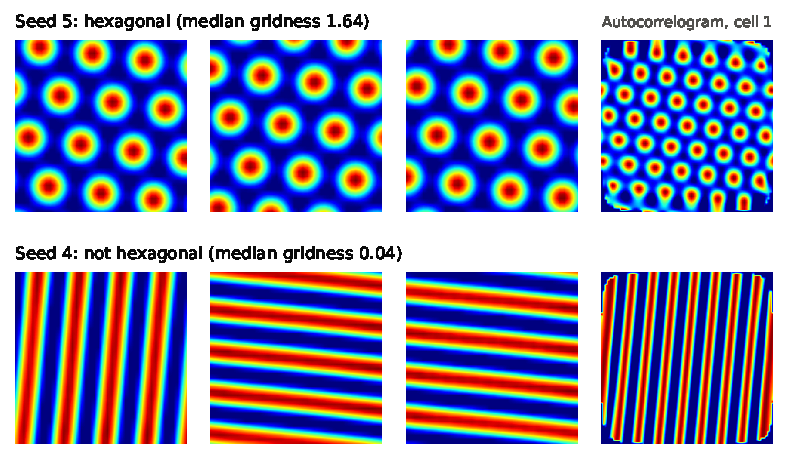
\includegraphics[width=0.8\linewidth]{figures/figA1_success_vs_failure.pdf}
  \caption{\looseness=-1 Learned firing patterns in our implementation, one run per row: (a) the reconstruction from the paper and its references, seed 5, hexagonal; (b) the same model, seed 4, parallel stripes; (c) the paper-text-only version, seed 1, a square lattice; (d, e) nonlinear model 1 (ReLU), built like (a), on two seeds. Each row shows three of the 24 learned cells (activity across the 1\,m arena; red is high, blue is low) and the spatial autocorrelogram of the first cell, with the run's median gridness. A hexagonal pattern gives six autocorrelogram peaks around the centre at 60$^\circ$ intervals, a square lattice four at 90$^\circ$, and stripes a set of parallel bands.}
  \label{fig:seeds}
\end{figure}

\begin{figure}[H]
  \captionsetup{margin=0.0in, font=sf}
  \centering
  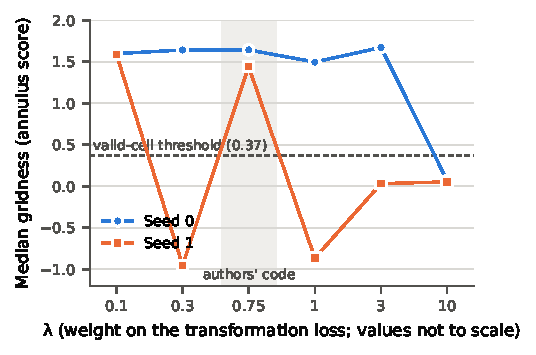
\includegraphics[width=0.55\linewidth]{figures/figA2_lambda_sweep.pdf}
  \caption{\looseness=-1 Median gridness over 24 cells against the loss weight $\lambda$ for the paper-text model, seeds 0 and 1. Points above the dashed line count as hexagonal. The shaded value, 0.75, is the effective weight in the authors' code.}
  \label{fig:lambda}
\end{figure}

\begin{figure}[H]
  \captionsetup{margin=0.0in, font=sf}
  \centering
  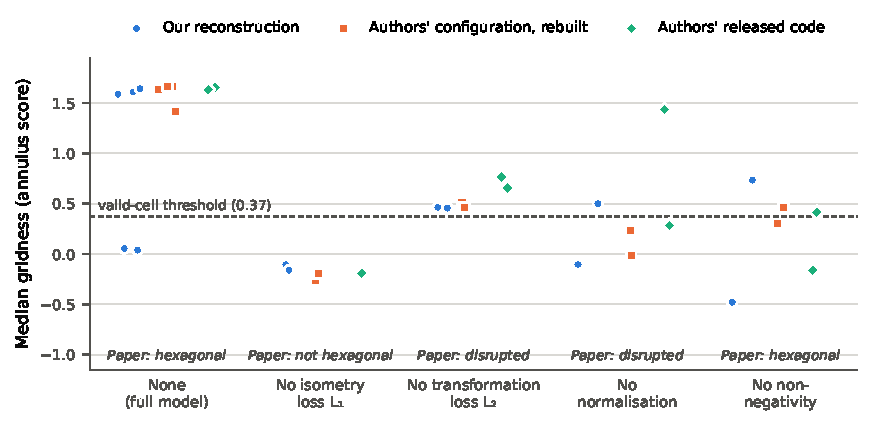
\includegraphics[width=0.9\linewidth]{figures/figA3_ablations.pdf}
  \caption{\looseness=-1 The paper's ablations (its Figure~3) repeated in three implementations: two seeds per ablation, and six, four and three seeds respectively for the full model. Each point is one run; points above the dashed line count as hexagonal. The paper's claim for each condition is printed beneath it.}
  \label{fig:ablations}
\end{figure}


\end{document}